%%%%%%%%%%%%%%%%%%%%%%%%%%%%%%%%%%%%%%%%%
% Short Sectioned Assignment LaTeX Template Version 1.0 (5/5/12)
% This template has been downloaded from: http://www.LaTeXTemplates.com
% Original author:  Frits Wenneker (http://www.howtotex.com)
% License: CC BY-NC-SA 3.0 (http://creativecommons.org/licenses/by-nc-sa/3.0/)
%%%%%%%%%%%%%%%%%%%%%%%%%%%%%%%%%%%%%%%%%

%----------------------------------------------------------------------------------------
%	PACKAGES AND OTHER DOCUMENT CONFIGURATIONS
%----------------------------------------------------------------------------------------

\documentclass[paper=a4]{article} % A4 paper and 11pt font size


\usepackage[hmargin=3.5cm]{geometry}
% ---- Entrada y salida de texto -----

\usepackage[T1]{fontenc} % Use 8-bit encoding that has 256 glyphs
\usepackage[utf8]{inputenc}

%\usepackage{fourier} % Use the Adobe Utopia font for the document - comment this line to return to the LaTeX default

% ---- Idioma --------

\usepackage[spanish, es-tabla]{babel} % Selecciona el español para palabras introducidas automáticamente, p.ej. "septiembre" en la fecha y especifica que se use la palabra Tabla en vez de Cuadro

% ---- Otros paquetes ----
\usepackage[hidelinks]{hyperref} % Estilo para los enlaces
\hypersetup{
  colorlinks   = true, %Colours links instead of ugly boxes
  urlcolor     = blue, %Colour for external hyperlinks
  linkcolor    = black, %Colour of internal links
  citecolor   = blue %Colour of citations
}
\usepackage{url} % ,href} %para incluir URLs e hipervínculos dentro del texto (aunque hay que instalar href)
\usepackage{amsmath,amsfonts,amsthm} % Math packages
%\usepackage{graphics,graphicx, floatrow} %para incluir imágenes y notas en las imágenes
\usepackage{graphics,graphicx, float} %para incluir imágenes y colocarlas
\usepackage{wrapfig}

%Para incluir codigo
%\usepackage{minted}
	
% Para hacer tablas comlejas
%\usepackage{multirow}
%\usepackage{threeparttable}

%\usepackage{sectsty} % Allows customizing section commands
%\allsectionsfont{\centering \normalfont\scshape} % Make all sections centered, the default font and small caps

\usepackage{fancyhdr} % Custom headers and footers
\pagestyle{fancyplain} % Makes all pages in the document conform to the custom headers and footers
\fancyhead{} % No page header - if you want one, create it in the same way as the footers below
\fancyfoot[L]{} % Empty left footer
\fancyfoot[C]{} % Empty center footer
\fancyfoot[R]{\thepage} % Page numbering for right footer
\renewcommand{\headrulewidth}{0pt} % Remove header underlines
\renewcommand{\footrulewidth}{0pt} % Remove footer underlines
\setlength{\headheight}{13.6pt} % Customize the height of the header

\numberwithin{equation}{section} % Number equations within sections (i.e. 1.1, 1.2, 2.1, 2.2 instead of 1, 2, 3, 4)
\numberwithin{figure}{section} % Number figures within sections (i.e. 1.1, 1.2, 2.1, 2.2 instead of 1, 2, 3, 4)
\numberwithin{table}{section} % Number tables within sections (i.e. 1.1, 1.2, 2.1, 2.2 instead of 1, 2, 3, 4)

\setlength\parindent{0pt} % Removes all indentation from paragraphs - comment this line for an assignment with lots of text

\newcommand{\horrule}[1]{\rule{\linewidth}{#1}} % Create horizontal rule command with 1 argument of height


%------------------------------------------------------------------------
%	TÍTULO Y DATOS DEL ALUMNO
%------------------------------------------------------------------------

\title{	
\normalfont \normalsize 
\textsc{\textbf{Modelos de Computación (2016-2017)} \\ Grado en Ingeniería Informática \\ Universidad de Granada} \\ [25pt] % Your university, school and/or department name(s)
\horrule{0.5pt} \\[0.4cm] % Thin top horizontal rule
\huge Autómatas Celulares \\ % The assignment title
\horrule{2pt} \\[0.5cm] % Thick bottom horizontal rule
}

\date{\normalsize\today} % Incluye la fecha actual

%-------------------------------------------------------------------------
% DOCUMENTO
%-------------------------------------------------------------------------

\begin{document}

\maketitle % Muestra el Título

\newpage

%-------------------------------------------------------------------------
%	Resumen introductorio (entre 5 y 15 lineas)
%----------------------------------------------------------------------
\begin{abstract} 
% INCOMPLETO!!!!!
Se ha realizado un trabajo sobre los autómatas celulares desarrollados en la época de los 60 por \textit{Von Neumann}. La teoría de los autómatas celulares ha ido cambiando durante su vida con diferentes vertientes y multitud de variaciones pero nos centraremos en solo dos versiones más a parte de la de Von Neumann.

% IDEA BASICA Y GENERAL - HAY QUE HACERLO BIEN!!!!!!!!

\end{abstract}

%--------------------------------------------------------------------------
%	Introducción
%-------------------------------------------------------------------------

\section{Introducción} % 
% http://web.archive.org/web/20080907225701/http://yupana.autonoma.edu.co/publicaciones/yupana/005/autocelular/Automatas.html

%

Para poder entender que son los autómatas celulares primero debemos comprender de donde viene la necesidad de crearlos, tanto a los propios autómatas como a su teoría que los sostiene. En la historia del ser humano y las ciencias se ha perseguido el modelamiento del mundo y todos sus fenómenos que ocurren en el, en concreto de los sistemas físicos, eléctricos y mecánicos mediante el uso de los modelos matemáticos. Matemáticamente hablando estos fenómenos de la naturales son sistemas de naturaleza continua y han sido tratados con ecuaciones diferenciales, integrales funcionales y variables de estado entre otros procedimientos matemáticos para su modelamiento. También están los modelos aproximados y discretos que ofrecen una teoría muy cercana a la realidad con la ventaja de utilizar valores finitos. Para ello se ha utilizado la discretización y la digitalización de sistemas.\\

Una de las técnicas matemáticas complejas para el modelado de sistemas físicos y mecánicos es el \textit{Método de los Elementos Finitos} (FEM), cuya finalidad es discretizar espacios de naturaleza contínua, sobre los cuales es posible realizar análisis numéricos para comprender, por medio de un modelo discreto, el comportamiento de sistemas analógicos. Pero esta técnica resulta muy compleja de aplicar por su dificultad para poder lograr modelos que describan sus comportamientos de forma precisa. Esta técnica (FEM) tiene una alta aplicación en el análisis de sistemas y espacios físicos-mecánicos donde el objetivo del modelo es comprender el comportamiento del sistema en el ambito de la resistencia de los materiales, la dinámica de partículas y en general el comportamiento con la interacción  de los elementos base del sistema en el espacio donde reside.
Aun así hay todavía un amplio grupo de sistemas que es imposible modelar con estas técnicas debido a diversos motivos, como por ejemplo, sistemas químicos, biológicos, evolutivos, eléctricos, computacionales e inclusive otros sistemas físicos y mecánicos. Para estos sistemas que no se podían modelar con FEM han aparecido a lo largo de la historia diferentes técnicas para obtener su modelo continuo, una de ellas fue el modelado con \textit{Autómata Celular}.




\section{Autómatas Celulares}
Aunque no existe una definición formal sobre que es un Autómata Celular entendemos que es estudio de modelado discreto para un sistema que evoluciona en generaciones o iteraciones discretas. Es recomendable utilizar esta técnica cuando se tiene un sistema con una colección masiva de objetos simples que interactúan unos con otros de forma aleatoria y por ello es utilizado en la teoría de la computación, las matemáticas, la física, las ciencias complejas, etc. \\

Un Autómata Celular consiste en una rejilla regular de celdas, donde cada celda se conoce como célula y representa un estado del conjunto de estados disponibles del sistema. Cada celda puede tomar un valor de un rango de valores definidos para este sistema en particular, siempre que el valor sea discreto y perteneciente al conjunto de los reales. Además cada celda viene definida por su ``vecindario'', entendemos por vecindario al conjunto finito de las células adyacentes a una célula en concreto.  La rejilla va cambiando en el tiempo y actualizando el estado de sus células, a cada instante de tiempo se le denomina generación y el estado de las células en una generación no varía.  \\


En el autómata celular cuando se avanza de generación, se actualiza el valor de todas las células del autómata aplicando una función de transición (``evolución''), que avanza el autómata al estado siguiente. Esta función de transición viene determinada por una ecuación matemática que toma como argumentos los valores de la vecindad de la célula además de del valor de la propia célula, siempre se aplica de forma homogénea y para cada paso discreto del tiempo.\\

Una manera de simular un autómata celular bidimensional es con una cuadricula de tamaño infinito. Cada célula tiene dos posible estados, blanco y negro. La vecindad de la célula se define por una regla en concreto, ya que la forma de considerar la adyacencia varía dependiendo del modelo y la versión del autómata que se utilice. Los tipos más comunes de vecindad son los que definieron el propio \textit{Neumann} y \textit{Moore} y que se apodaron igual que sus autores. El vecindario definido por \textit{Von Neumann} se define como el conjunto de cuatro células que rodean ortogonalmente a una célula central, hay una variante de este vecindario que es una variante de este, la zona ampliada de \textit{Von Neumann} que consiste en ampliar el vecindario a las ocho células que rodean ortogonalmente a la célula central. El vecindario definido por \textit{Moore} consiste en las ocho células adyacentes que rodean a una célula central.\\


\begin{figure}[H]
\centering
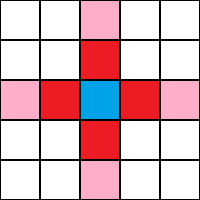
\includegraphics[scale=0.5]{imagenes/CA_Neumann.png}
\hspace{2cm}
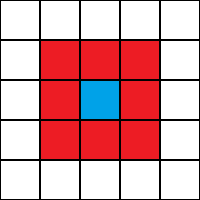
\includegraphics[scale=0.5]{imagenes/CA-Moore.png}
\caption{Vecindad en color rojo de la célula azul de forma gráfica, izquierda vecindad ampliada de Von Neumann y derecha vecindad de Moore}
\label{fig:vecindad}

\end{figure}

La ecuación general para el sistemas de reglas que se utiliza para determinar el estado de la célula en la generación siguiente es del tipo $k^{k^s}$ donde $k$ es el número de posibles estados para una célula, y $s$ es el número de células de la vecindad (incluyendo al propia célula) 

Hola \cite{Teoria_von_neumann} hola
\subsection{Historia}


%--------------------------------------------------------------------------
%	Era de Von Neumann
%--------------------------------------------------------------------------

\section{Era de Von Neumann} % 

%--------------------------------------------------------------------------
%	Era de John Horton Conway
%--------------------------------------------------------------------------

\section{Era de John Horton Conway} % 


%--------------------------------------------------------------------------
%	Era de Stephen Wolfram
%--------------------------------------------------------------------------

\section{Era de Stephen Wolfram} % 

%--------------------------------------------------------------------------
%	Aplicaciones Actuales 
%--------------------------------------------------------------------------

\section{Aplicaciones Actuales} % 

\subsection{Modelado de flujo de tráfico y peatones}

\subsection{Modelado de evolución de células o virus}

%------------------------------------------------

\bibliography{citas} %archivo citas.bib que contiene las entradas 
\bibliographystyle{plain} % hay varias formas de citar

\end{document}



